\documentclass[10pt]{beamer}

\usepackage[utf8x]{inputenc}
\usepackage[english]{babel}
\usepackage{amsmath, amsfonts, amssymb}
\usepackage{color}
\usepackage{xcolor}
\usepackage{tikz}
\usetikzlibrary{positioning,shapes,shadows,arrows,snakes}
\usepackage{listliketab}
\usepackage{shuffle}
\usepackage{xargs}
\usepackage{multirow}
\usepackage{pgfplots}
\usepackage{csquotes}
\usepackage{verbatim}

\definecolor{BlueGreen}{cmyk}{0.85,0,0.33,0}
\definecolor{RawSienna}{cmyk}{0,0.72,1,0.45}
\definecolor{gold}{rgb}{1.,0.84,0.}
\definecolor{dgreen}{rgb}{0.,0.6,0.}

\definecolor{Noir}{RGB}{0,0,0}
\definecolor{Rouge}{RGB}{205,35,38}
\definecolor{Bleu}{RGB}{2,60,195}
\definecolor{Bleu1}{RGB}{121,176,197}
\definecolor{Vert}{RGB}{23,103,1}
\definecolor{VertOlive}{RGB}{112,141,35}
\definecolor{Orange}{RGB}{255,113,15}
\definecolor{RoseBonbon}{RGB}{249,66,158}
\definecolor{Marron}{RGB}{193,88,50}

\definecolor{mygreen}{RGB}{23,103,1}

\newcommand{\red}[1]{\textcolor{red}{#1}}
\newcommand{\blue}[1]{\textcolor{blue}{#1}}
\newcommand{\green}[1]{\textcolor{mygreen}{#1}}
\newcommand{\bluealert}[2]{\textcolor<#1>{blue}{#2}}

\tikzstyle{alert} = [color=red, line width = 1.5]
\tikzstyle{bluealert} = [color=blue, line width =1.5]
\tikzstyle{big} = [line width = 1.5]
\tikzstyle{Point} = [fill, radius=0.08]
\tikzstyle{RedPoint} = [fill, radius=0.09, color = red]


\tikzstyle{Red} = [color = red]
\tikzstyle{Blue} = [color = blue]
\tikzstyle{Green} = [color = Vert]
\tikzstyle{Gray} = [color = gray]

\definecolor{violet}{rgb}{.5,.1,.9}


\usetheme{Boadilla}
\title{Learning methods for limited datasets}
\author[G. Châtel]{Grégory Châtel\\\vspace{0.3cm}Disaitek\\Intel AI Software Innovator\\\vspace{0.3cm}gchatel@disaitek.com\\@rodgzilla\\github.com/rodgzilla}
\date{November 21st, 2018}

\setbeamertemplate{footline}[frame number]{}
\setbeamertemplate{navigation symbols}{}

%% \usebackgroundtemplate{
%%   \includegraphics[width=\paperwidth,height=\paperheight]{images/logo_disaitek.png}
%% }

%% \usebackgroundtemplate{
%%   \rule{-4.5cm}{\paperheight}
%%   \hspace*{\paperwidth}
%%   \makebox[0pt][r]{
%%     %% \scalebox{0.7}{
%%       \includegraphics[width=\paperwidth,height=\paperheight]{images/logo_disaitek.png}
%%     %% }
%%   }
%% }

\begin{document}

%%%%%%%%%%%%%%%%%%%%%%%%%%%%%%%%%%%%%%%%%%%%%%%%%%%%%%%%%%%%%%%%%%%%%%
\begin{frame}

  \maketitle

\end{frame}
%%%%%%%%%%%%%%%%%%%%%%%%%%%%%%%%%%%%%%%%%%%%%%%%%%%%%%%%%%%%%%%%%%%%%%

%%%%%%%%%%%%%%%%%%%%%%%%%%%%%%%%%%%%%%%%%%%%%%%%%%%%%%%%%%%%%%%%%%%%%%
\begin{frame}

  \tableofcontents

\end{frame}
%%%%%%%%%%%%%%%%%%%%%%%%%%%%%%%%%%%%%%%%%%%%%%%%%%%%%%%%%%%%%%%%%%%%%%

\section{Introduction}

%%%%%%%%%%%%%%%%%%%%%%%%%%%%%%%%%%%%%%%%%%%%%%%%%%%%%%%%%%%%%%%%%%%%%%
\begin{frame}

  \frametitle{Machine learning}

  \framesubtitle{Supervised learning}

  Machine learning is a subfield of artificial intelligence.

  \bigskip

  \begin{center}
    \scalebox{0.6}{
      \input{figures/scatter.tex}
    }
  \end{center}

  \begin{description}
    \item[Intuitively] We want to \emph{learn from} and \emph{make predictions
    on} data.

    \medskip

    \item[Technically] We want to build a model that approximate well
      (\textit{e.g.} minimize a loss function) an unknown function for
      which we only have limited observations.
  \end{description}

  \bigskip

  To do this, we usually need \emph{a lot of data}.

\end{frame}
%%%%%%%%%%%%%%%%%%%%%%%%%%%%%%%%%%%%%%%%%%%%%%%%%%%%%%%%%%%%%%%%%%%%%%o

%%%%%%%%%%%%%%%%%%%%%%%%%%%%%%%%%%%%%%%%%%%%%%%%%%%%%%%%%%%%%%%%%%%%%%
\begin{frame}
  \frametitle{Neural network}

  \framesubtitle{Neuron with activation}

  \begin{center}
    \scalebox{0.6}{
      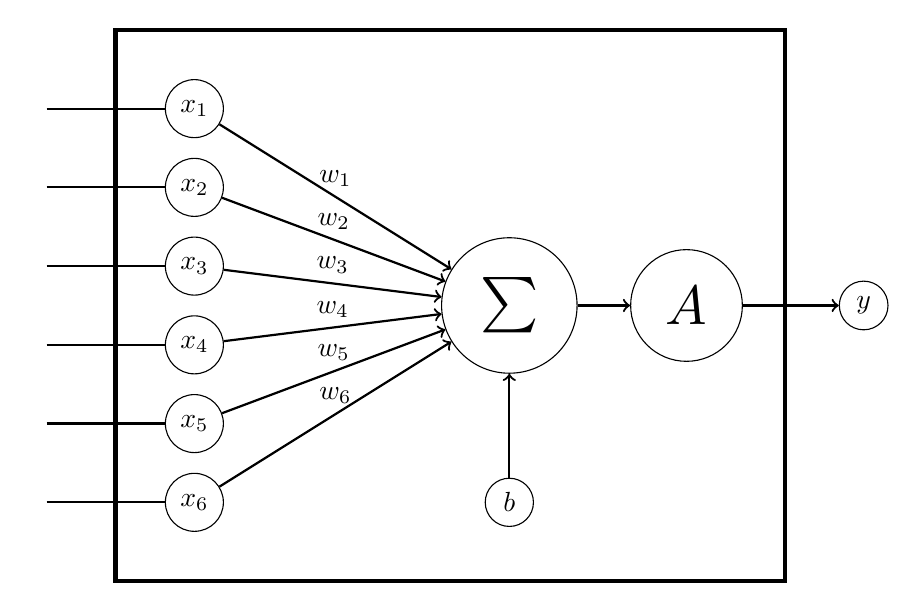
\begin{tikzpicture}
  \node (f1) at (-2, 0) {};

  \node[draw, circle] (X1) at (0, 0){
    $x_{1}$
  };

  \node (f2) at (-2, -1) {};

  \node[draw, circle] (X2) at (0, -1){
    $x_{2}$
  };

  \node (f3) at (-2, -2) {};

  \node[draw, circle] (X3) at (0, -2){
    $x_{3}$
  };

  \node (f4) at (-2, -3) {};

  \node[draw, circle] (X4) at (0, -3){
    $x_{4}$
  };

  \node (f5) at (-2, -4) {};

  \node[draw, circle] (X5) at (0, -4){
    $x_{5}$
  };

  \node (f6) at (-2, -5) {};

  \node[draw, circle] (X6) at (0, -5){
    $x_{6}$
  };

  \node[draw, circle] (bias) at (4, -5){
    $b$
  };

  \node[draw, circle] (sum) at (4, -2.5){
    \scalebox{2}{
      $\sum$
    }
  };

  \node[draw, circle] (activation) at (6.25, -2.5){
    \scalebox{2}{
      $A$
    }
  };


  %% \uncover<2->{
  %%   \node[draw, circle] (activation) at (6.25, -2.5){
  %%     \scalebox{2}{
  %%       $A$
  %%     }
  %%   };
  %% }

  \node[draw, circle] (y) at (8.5, -2.5){
    $y$
  };

  \draw[thick] (f1) -- (X1);
  \draw[thick] (f2) -- (X2);
  \draw[thick] (f3) -- (X3);
  \draw[thick] (f4) -- (X4);
  \draw[thick] (f5) -- (X5);
  \draw[thick] (f6) -- (X6);

  \draw[thick, ->] (X1) -- node [above]{$w_{1}$} (sum);
  \draw[thick, ->] (X2) -- node [above]{$w_{2}$} (sum);
  \draw[thick, ->] (X3) -- node [above]{$w_{3}$} (sum);
  \draw[thick, ->] (X4) -- node [above]{$w_{4}$} (sum);
  \draw[thick, ->] (X5) -- node [above]{$w_{5}$} (sum);
  \draw[thick, ->] (X6) -- node [above]{$w_{6}$} (sum);
  \draw[thick, ->] (bias) -- (sum);
  %% \uncover<1>{
  %%   \draw[thick, ->] (sum) -- (y);
  %% }
  %% \uncover<2->{
  %%   \draw[thick, ->] (sum) -- (activation);
  %%   \draw[thick, ->] (activation) -- (y);
  %% }
  \draw[thick, ->] (sum) -- (activation);
  \draw[thick, ->] (activation) -- (y);

  \path [ultra thick, draw] (-1, 1) -- (7.5, 1) rectangle (-1, -6) -- (7.5, -6);
\end{tikzpicture}

    }
  \end{center}

  \begin{center}
    \scalebox{0.8}{
      \begin{tikzpicture}[xscale = 4]
        \node (formula) (0, 0){
          \scalebox{1.3}{
            $A(x) = \frac{1}{1 + e^{-x}}$
          }
        } ;

        \node (graph) at (1, 0){
          \scalebox{0.6}{
            \begin{tikzpicture}
  \begin{axis}[
      legend pos=north west,
      axis x line=middle,
      axis y line=middle,
      x tick label style={/pgf/number format/fixed,
        /pgf/number format/fixed zerofill,
        /pgf/number format/precision=1},
      y tick label style={/pgf/number format/fixed,
        /pgf/number format/fixed zerofill,
        /pgf/number format/precision=1},
      grid = major,
      width=7cm,
      height=5cm,
      grid style={dashed, gray!30},
      xmin=-8,     % start the diagram at this x-coordinate
      xmax= 8,    % end   the diagram at this x-coordinate
      ymin= -0.2,     % start the diagram at this y-coordinate
      ymax= 1.2,   % end   the diagram at this y-coordinate
      %axis background/.style={fill=white},
      xlabel=x,
      ylabel=y,
      tick align=outside,
      enlargelimits=false]
    % plot the stirling-formulae
    \addplot[domain=-8:8, red, thick,samples=500] {1/(1+exp(-x))};
  \end{axis}
\end{tikzpicture}

          }
        };
      \end{tikzpicture}
    }
  \end{center}

  \vspace{-0.5cm}

  \[
  y = A(w_{1}x_{1} + w_{2}x_{2} + w_{3}x_{3} + w_{4}x_{4} + w_{5}x_{5} + w_{6}x_{6} + b)
  \]
\end{frame}
%%%%%%%%%%%%%%%%%%%%%%%%%%%%%%%%%%%%%%%%%%%%%%%%%%%%%%%%%%%%%%%%%%%%%%

%%%%%%%%%%%%%%%%%%%%%%%%%%%%%%%%%%%%%%%%%%%%%%%%%%%%%%%%%%%%%%%%%%%%%%
\begin{frame}
  \frametitle{Neural network}

  \framesubtitle{Network}

  \begin{center}
    \scalebox{0.7}{
      \input{figures/network_animation.tex}
    }
  \end{center}
\end{frame}
%%%%%%%%%%%%%%%%%%%%%%%%%%%%%%%%%%%%%%%%%%%%%%%%%%%%%%%%%%%%%%%%%%%%%%

%%%%%%%%%%%%%%%%%%%%%%%%%%%%%%%%%%%%%%%%%%%%%%%%%%%%%%%%%%%%%%%%%%%%%%
\begin{frame}
  \frametitle{Neural network}

  \framesubtitle{Training}

  \begin{center}
    \scalebox{0.5}{
      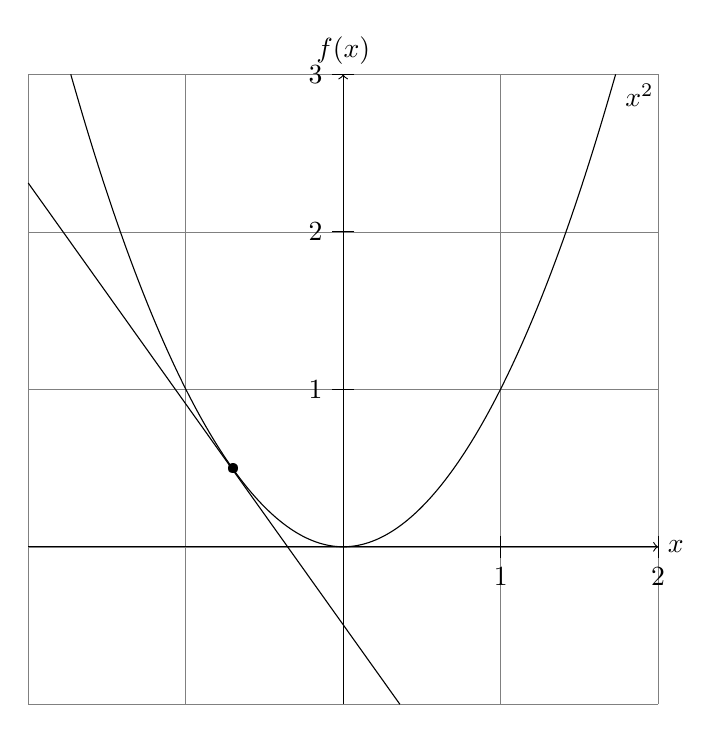
\begin{tikzpicture}[scale=2]
%  \draw[style=help lines] (0,0) grid (3.9,3.9);$
  \draw[style=help lines] (-2,-1) grid (2,3);

  \draw[->] (-2,0) -- (2,0) node[right] {$x$};
  \draw[->] (0,-1) -- (0,3) node[above] {$f(x)$};

  \foreach \x/\xtext in {1/1, 2/2}
    \draw[shift={(\x,0)}] (0pt,2pt) -- (0pt,-2pt) node[below] {$\xtext$};

  \foreach \y/\ytext in {1/1, 2/2, 3/3}
    \draw[shift={(0,\y)}] (2pt,0pt) -- (-2pt,0pt) node[left] {$\ytext$};

  \draw (-1.73,3) parabola bend (0,0) (1.73,3) node[below right] {$x^2$};
  \node at (-0.7, 0.49) {
    \textbullet
  };
  \draw (-2, 2.31) -- (0.36, -1);
\end{tikzpicture}

%% \begin{tikzpicture}[scale=2]
%%   \shade[top color=blue,bottom color=gray!50]
%%       (0,0) parabola (1.5,2.25) |- (0,0);
%%   \draw (1.05cm,2pt) node[above]
%%       {$\displaystyle\int_0^{3/2} \!\!x^2\mathrm{d}x$};

%%   \draw[style=help lines] (0,0) grid (3.9,3.9)
%%        [step=0.25cm]      (1,2) grid +(1,1);

%%   \draw[->] (-0.2,0) -- (4,0) node[right] {$x$};
%%   \draw[->] (0,-0.2) -- (0,4) node[above] {$f(x)$};

%%   \foreach \x/\xtext in {1/1, 1.5/1\frac{1}{2}, 2/2, 3/3}
%%     \draw[shift={(\x,0)}] (0pt,2pt) -- (0pt,-2pt) node[below] {$\xtext$};

%%   \foreach \y/\ytext in {1/1, 2/2, 2.25/2\frac{1}{4}, 3/3}
%%     \draw[shift={(0,\y)}] (2pt,0pt) -- (-2pt,0pt) node[left] {$\ytext$};

%%   \draw (-.5,.25) parabola bend (0,0) (2,4) node[below right] {$x^2$};
%% \end{tikzpicture}

    }
  \end{center}

  \smallskip

  A differentiable loss function $L(\theta, x, y)$ tells us how well
  the model is performing. We compute how parameters changes influence
  the loss by taking its gradient $\nabla_{\theta} L(\theta, x, y)$.

  \medskip

  We then update the weights to make the value of the loss function
  decrease by iterating this formula:

  \[
  \theta_{t + 1} = \theta_{t} - \alpha \nabla_{\theta_{t}} L(\theta_{t}, x, y).
  \]
\end{frame}
%%%%%%%%%%%%%%%%%%%%%%%%%%%%%%%%%%%%%%%%%%%%%%%%%%%%%%%%%%%%%%%%%%%%%%

\section{Popular ML tasks and their dataset}

%%%%%%%%%%%%%%%%%%%%%%%%%%%%%%%%%%%%%%%%%%%%%%%%%%%%%%%%%%%%%%%%%%%%%%
\begin{frame}

  \frametitle{Popular datasets}

  \framesubtitle{Computer vision}

  \begin{description}[labelwidth=\widthof{bf series 2017, JFT-300M}]
    \setlength{\itemsep}{8pt}
    \item[1990, Statlog] $\sim$2k outdoor images,
    \item[1998, MNIST] 60k B\&W images of handwritten digits,
    \item[2005, LabelMe] $\sim$187k scenes images,
    \item[2009, ImageNet] $\sim$14M images with 1000 different categories,
    \item[2017, JFT-300M] $\sim$300M RGB images $\sim$18k categories (internal dataset @ Google).
  \end{description}

\end{frame}
%%%%%%%%%%%%%%%%%%%%%%%%%%%%%%%%%%%%%%%%%%%%%%%%%%%%%%%%%%%%%%%%%%%%%%

%%%%%%%%%%%%%%%%%%%%%%%%%%%%%%%%%%%%%%%%%%%%%%%%%%%%%%%%%%%%%%%%%%%%%%
\begin{frame}

  \frametitle{Popular datasets}

  \framesubtitle{Natural language processing (NLP)}

  \begin{description}[labelwidth=\widthof{bf series 2017, JFT-300M}]
    \setlength{\itemsep}{8pt}
    \item[1997, Car evaluation dataset] $\sim$2k textual car evaluations,
    \item[2005, Stanford Sentiment Treebank] $\sim$11k movie reviews,
    \item[2011, IMDB Reviews] $\sim$50k movie reviews,
    \item[2012, Youtube Comedy Slam] $\sim$1.1M pairs of video metadata,
    \item[2015, Amazon reviews] $\sim$82M product reviews.
  \end{description}

\end{frame}
%%%%%%%%%%%%%%%%%%%%%%%%%%%%%%%%%%%%%%%%%%%%%%%%%%%%%%%%%%%%%%%%%%%%%%

%%%%%%%%%%%%%%%%%%%%%%%%%%%%%%%%%%%%%%%%%%%%%%%%%%%%%%%%%%%%%%%%%%%%%%
\begin{frame}

  \frametitle{Creating dataset}

  Creating new high quality datasets is both \textcolor{blue}{hard}
  and \textcolor{blue}{expensive}.

  \bigskip

  Some researchers experiment with training models using
  \textcolor{blue}{low quality data} (weakly supervised learning).

  \bigskip

  Amazon offers a \textcolor{blue}{dataset creation service} (Amazon
  Mechanical Turk) where you can pay to get your dataset labelled by
  humans.

\end{frame}
%%%%%%%%%%%%%%%%%%%%%%%%%%%%%%%%%%%%%%%%%%%%%%%%%%%%%%%%%%%%%%%%%%%%%%

\section{Data efficiency}

%%%%%%%%%%%%%%%%%%%%%%%%%%%%%%%%%%%%%%%%%%%%%%%%%%%%%%%%%%%%%%%%%%%%%%
\begin{frame}
  \frametitle{Data efficiency}

  Knowing that datasets are so important and hard to create, it is
  important to squeeze \emph{every last bit of value} out of them.

  \bigskip

  To do this, three ideas are explored:

  \begin{itemize}
    \item Transfer learning,
    \item Multi-task learning,
    \item Semi-supervised learning.
  \end{itemize}

\end{frame}
%%%%%%%%%%%%%%%%%%%%%%%%%%%%%%%%%%%%%%%%%%%%%%%%%%%%%%%%%%%%%%%%%%%%%%

\subsection{Transfer learning}

%%%%%%%%%%%%%%%%%%%%%%%%%%%%%%%%%%%%%%%%%%%%%%%%%%%%%%%%%%%%%%%%%%%%%%
\begin{frame}

  \frametitle{Transfer learning}

  \framesubtitle{Concept}

  \begin{displayquote}[Perkins, 1992]
  The application of skills, knowledge, and/or attitudes that were
  learned in one situation to another learning situation.
  \end{displayquote}

  \bigskip

  Transfer learning consists in taking an artificial neural network
  that has been trained on a \textcolor{blue}{\emph{generic}} task and
  \textcolor{blue}{\emph{transferring}} its knowledge (retraining it)
  to perform a new task.

  \bigskip

  The idea behind this method is that the information learned on a
  generic task will probably be useful for a new task of the same
  domain.

  \bigskip

  Transfer learning is actually the base of the
  \textcolor{blue}{Google Cloud AutoML service}.

\end{frame}
%%%%%%%%%%%%%%%%%%%%%%%%%%%%%%%%%%%%%%%%%%%%%%%%%%%%%%%%%%%%%%%%%%%%%%

%%%%%%%%%%%%%%%%%%%%%%%%%%%%%%%%%%%%%%%%%%%%%%%%%%%%%%%%%%%%%%%%%%%%%%
\begin{frame}

  \frametitle{Transfer learning}

  \framesubtitle{Computer vision}

  \begin{center}
    \includegraphics[width = 7cm]{images/alexnet_architecture.png}
  \end{center}

  Using this trained model as a base to build a dogs vs cats picture
  classifier \textcolor{blue}{greatly reduce the need of labelled
    data}.

  \bigskip

  The knowledge about \textcolor{blue}{basic shapes and textures} that
  has been learned on ImageNet will be useful to almost all task
  involving real world images.

\end{frame}
%%%%%%%%%%%%%%%%%%%%%%%%%%%%%%%%%%%%%%%%%%%%%%%%%%%%%%%%%%%%%%%%%%%%%%

%%%%%%%%%%%%%%%%%%%%%%%%%%%%%%%%%%%%%%%%%%%%%%%%%%%%%%%%%%%%%%%%%%%%%%
\begin{frame}

  \frametitle{Transfer learning}

  \framesubtitle{Natural language processing}

  \begin{center}
    \scalebox{0.7}{
      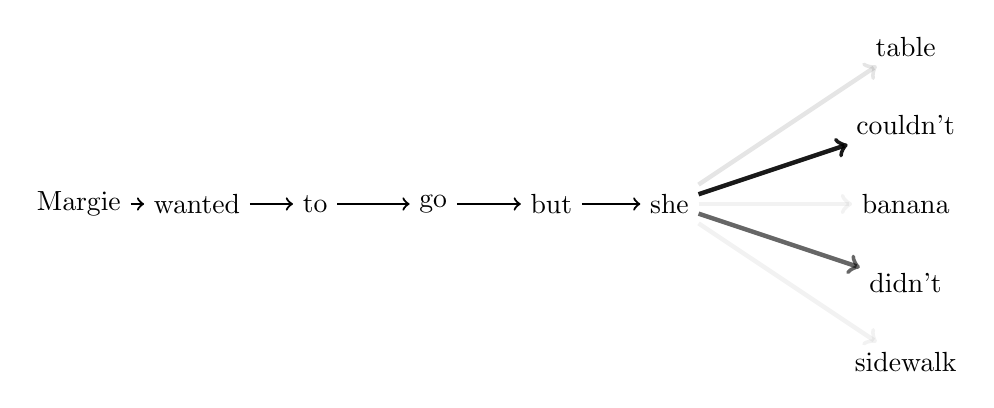
\begin{tikzpicture}[xscale = 1.5]
  \node (W1) at (0, 0) {
    Margie
  };


  \node (W2) at (1, 0) {
    wanted
  };

  \node (W3) at (2, 0) {
    to
  };

  \node (W4) at (3, 0) {
    go
  };

  \node (W5) at (4, 0) {
    but
  };

  \node (W6) at (5, 0) {
    she
  };

  \node (W7) at (7, 2) {
    table
  };

  \node (W8) at (7, 1) {
    couldn't
  };

  \node (W9) at (7, 0) {
    banana
  };

  \node (W10) at (7, -1) {
    didn't
  };

  \node (W11) at (7, -2) {
    sidewalk
  };

  \draw[thick, ->] (W1) -- (W2);
  \draw[thick, ->] (W2) -- (W3);
  \draw[thick, ->] (W3) -- (W4);
  \draw[thick, ->] (W4) -- (W5);
  \draw[thick, ->] (W5) -- (W6);
  \draw[ultra thick, ->, opacity = 0.1] (W6) -- (W7);
  \draw[ultra thick, ->, opacity = 0.9] (W6) -- (W8);
  \draw[ultra thick, ->, opacity = 0.05] (W6) -- (W9);
  \draw[ultra thick, ->, opacity = 0.6] (W6) -- (W10);
  \draw[ultra thick, ->, opacity = 0.05] (W6) -- (W11);
\end{tikzpicture}

    }
  \end{center}

  The \textcolor{blue}{language modeling task} is currently the most
  generic task that NLP researcher have found to perform transfer
  learning.

  \bigskip

  Knowing how to predict the most likely following word requires to
  understand, to some extent, the \textcolor{blue}{meaning of words},
  \textcolor{blue}{the syntax of the language} and
  \textcolor{blue}{the way concepts interact}.

  \bigskip

  Typical language models are trained on Wikipedia content, books or
  Internet Common Crawl.

\end{frame}
%%%%%%%%%%%%%%%%%%%%%%%%%%%%%%%%%%%%%%%%%%%%%%%%%%%%%%%%%%%%%%%%%%%%%%

\subsection{Multi-task learning}

%%%%%%%%%%%%%%%%%%%%%%%%%%%%%%%%%%%%%%%%%%%%%%%%%%%%%%%%%%%%%%%%%%%%%%
\begin{frame}
  \frametitle{Multi-task learning}

  \framesubtitle{Concept}

  \bigskip

  %% \begin{displayquote}[Rich Caruana, 1997]
  %%   Multitask Learning is an approach to inductive transfer that
  %%   improves generalization by using the domain information contained
  %%   in the training signals of related tasks as an inductive bias. It
  %%   does this by learning tasks in parallel while using a shared
  %%   representation; what is learned for each task can help other tasks
  %%   be learned better.
  %% \end{displayquote}

  \begin{displayquote}[Rich Caruana, 1997]
    Multi-task learning is an approach to inductive transfer that
    improves generalization [...] It
    does this by learning tasks in parallel while using a shared
    representation; what is learned for each task can help other tasks
    be learned better.
  \end{displayquote}

  \bigskip

  Instead of just training the network to perform the desired task, we
  also optimize it to perform \textcolor{blue}{\emph{auxiliary
      tasks}}.

  \begin{center}
    \includegraphics[width = 4.5cm]{images/multi_task_learning.png}
  \end{center}

  {\scriptsize \textit{Image from http://ruder.io/multi-task/}}
\end{frame}
%%%%%%%%%%%%%%%%%%%%%%%%%%%%%%%%%%%%%%%%%%%%%%%%%%%%%%%%%%%%%%%%%%%%%%

%%%%%%%%%%%%%%%%%%%%%%%%%%%%%%%%%%%%%%%%%%%%%%%%%%%%%%%%%%%%%%%%%%%%%%
\begin{frame}
  \frametitle{Multi-task learning}

  \framesubtitle{Regularization technique}

  \begin{center}
    \includegraphics[width = 8cm]{images/overfitting.png}
  \end{center}

  Informally, the goal of the multi-task learning is to force the
  model to use its \textcolor{blue}{computing power} to perform
  something \textcolor{blue}{meaningful} instead of using it to learn
  the \textcolor{blue}{noise} of the data (overfitting).

  \bigskip

  {\scriptsize \textit{Image from
      https://hackernoon.com/memorizing-is-not-learning-6-tricks-to-prevent-overfitting-in-machine-learning-820b091dc42}}
\end{frame}
%%%%%%%%%%%%%%%%%%%%%%%%%%%%%%%%%%%%%%%%%%%%%%%%%%%%%%%%%%%%%%%%%%%%%%

%%%%%%%%%%%%%%%%%%%%%%%%%%%%%%%%%%%%%%%%%%%%%%%%%%%%%%%%%%%%%%%%%%%%%
\begin{frame}
  \frametitle{Multi-task learning}

  \framesubtitle{Computer vision}

  \begin{center}
    \includegraphics[width = 5.cm]{images/multi_task_medecine.png}
  \end{center}

  \medskip

  Some researchers discovered that by asking a model to predict the
  gender and age of patient in addition to detect \emph{cardiovascular
    diseases} they got strong performance improvements.

  \medskip

  {\scriptsize Poplin, Ryan, et al. "Predicting cardiovascular risk
    factors from retinal fundus photographs using deep learning."
    arXiv preprint arXiv:1708.09843 (2017).}
\end{frame}
%%%%%%%%%%%%%%%%%%%%%%%%%%%%%%%%%%%%%%%%%%%%%%%%%%%%%%%%%%%%%%%%%%%%%%

%%%%%%%%%%%%%%%%%%%%%%%%%%%%%%%%%%%%%%%%%%%%%%%%%%%%%%%%%%%%%%%%%%%%%%
\begin{frame}
  \frametitle{Multi-task learning}

  \framesubtitle{Natural language processing}

  \begin{center}
    \includegraphics[width = 4cm]{images/multi_task_nlp.png}
  \end{center}

  In NLP, translation can be used as an auxiliary task to improve
  models that perform tasks that have relatively small datasets such
  as sentence parsing.

  \bigskip

  By making the model perform translation, a task with huge datasets,
  we allow it to gain access to a much richer
  \textcolor{blue}{structure of the language}.

  \bigskip

  {\scriptsize Kaiser, Lukasz, et al. "One model to learn them all."
    arXiv preprint arXiv:1706.05137 (2017).}

\end{frame}
%%%%%%%%%%%%%%%%%%%%%%%%%%%%%%%%%%%%%%%%%%%%%%%%%%%%%%%%%%%%%%%%%%%%%%

\subsection{Semi-supervised learning}

%%%%%%%%%%%%%%%%%%%%%%%%%%%%%%%%%%%%%%%%%%%%%%%%%%%%%%%%%%%%%%%%%%%%%%
\begin{frame}

  \frametitle{Semi-supervised learning}

  \framesubtitle{Concept}

  \begin{center}
    \includegraphics[width=4cm]{images/semi_supervised_learning.png}
  \end{center}

  \bigskip

  The idea of semi-supervised learning is to use
  \textcolor{blue}{\emph{unlabelled data}} to improve our model.

  \bigskip

  {\scriptsize \textit{Image from https://en.wikipedia.org/wiki/Semi-supervised\_learning}}
\end{frame}
%%%%%%%%%%%%%%%%%%%%%%%%%%%%%%%%%%%%%%%%%%%%%%%%%%%%%%%%%%%%%%%%%%%%%%

%%%%%%%%%%%%%%%%%%%%%%%%%%%%%%%%%%%%%%%%%%%%%%%%%%%%%%%%%%%%%%%%%%%%%%
\begin{frame}

  \frametitle{Semi-supervised learning}

  \framesubtitle{Concept}

  The main concept of semi-supervised learning is to train a
  \textcolor{blue}{weaker student} to imitate a
  \textcolor{blue}{stronger teacher}.

  \bigskip

  Technically, we apply \emph{mean-squared error} or a
  \emph{Kullback-Liebler divergence} between the logits output by the
  student and the teacher. We typically alternate between supervised
  and semi-supervised steps of training.

  \bigskip

  The goal of this method is to \textcolor{blue}{propagate labels} and
  improve \textcolor{blue}{noise invariance}.

\end{frame}
%%%%%%%%%%%%%%%%%%%%%%%%%%%%%%%%%%%%%%%%%%%%%%%%%%%%%%%%%%%%%%%%%%%%%%

%%%%%%%%%%%%%%%%%%%%%%%%%%%%%%%%%%%%%%%%%%%%%%%%%%%%%%%%%%%%%%%%%%%%%%
\begin{frame}
  \frametitle{Semi-supervised learning}

  \framesubtitle{Computer vision}

  \begin{center}
    \begin{tikzpicture}
  \node (cleanImage) at (0, 0) {
    \includegraphics[width = 1.4cm]{images/dog_clean.jpg}
  };

  \node (perturbedImage) at (2.5, -2) {
    \includegraphics[width = 1.4cm]{images/dog_perturbation.jpg}
  };

  \node (teacher) at (5, 2) {
    \scalebox{0.15}{
      \begin{tikzpicture}[xscale = 3]
  \node[draw, circle] (N11) at (0, 0){
  };

  \node[draw, circle] (N21) at (0, -1){
  };

  \node[draw, circle] (N31) at (0, -2){
  };

  \node[draw, circle] (N41) at (0, -3){
  };

  \node[draw, circle] (N51) at (0, -4){
  };

  \node[draw, circle] (N61) at (0, -5){
  };

  \node[draw, circle] (N71) at (0, -6){
  };

  \node[draw, circle] (N81) at (0, -7){
  };

  \node[draw, circle] (N91) at (0, -8){
  };

  \node[draw, circle] (N12) at (1, 0){
  };

  \node[draw, circle] (N22) at (1, -1){
  };

  \node[draw, circle] (N32) at (1, -2){
  };

  \node[draw, circle] (N42) at (1, -3){
  };

  \node[draw, circle] (N52) at (1, -4){
  };

  \node[draw, circle] (N62) at (1, -5){
  };

  \node[draw, circle] (N72) at (1, -6){
  };

  \node[draw, circle] (N82) at (1, -7){
  };

  \node[draw, circle] (N92) at (1, -8){
  };

  \node[draw, circle] (N13) at (2, 0){
  };

  \node[draw, circle] (N23) at (2, -1){
  };

  \node[draw, circle] (N33) at (2, -2){
  };

  \node[draw, circle] (N43) at (2, -3){
  };

  \node[draw, circle] (N53) at (2, -4){
  };

  \node[draw, circle] (N63) at (2, -5){
  };

  \node[draw, circle] (N73) at (2, -6){
  };

  \node[draw, circle] (N83) at (2, -7){
  };

  \node[draw, circle] (N93) at (2, -8){
  };

  \node[draw, circle] (N14) at (3, -3.5){
  };

  \node[draw, circle] (N24) at (3, -4.5){
  };

  \draw[->] (N11) -- (N12);
  \draw[->] (N11) -- (N22);
  \draw[->] (N11) -- (N32);
  \draw[->] (N11) -- (N42);
  \draw[->] (N11) -- (N52);
  \draw[->] (N11) -- (N62);
  \draw[->] (N11) -- (N72);
  \draw[->] (N11) -- (N82);
  \draw[->] (N11) -- (N92);
  \draw[->] (N21) -- (N12);
  \draw[->] (N21) -- (N22);
  \draw[->] (N21) -- (N32);
  \draw[->] (N21) -- (N42);
  \draw[->] (N21) -- (N52);
  \draw[->] (N21) -- (N62);
  \draw[->] (N21) -- (N72);
  \draw[->] (N21) -- (N82);
  \draw[->] (N21) -- (N92);
  \draw[->] (N31) -- (N12);
  \draw[->] (N31) -- (N22);
  \draw[->] (N31) -- (N32);
  \draw[->] (N31) -- (N42);
  \draw[->] (N31) -- (N52);
  \draw[->] (N31) -- (N62);
  \draw[->] (N31) -- (N72);
  \draw[->] (N31) -- (N82);
  \draw[->] (N31) -- (N92);
  \draw[->] (N41) -- (N12);
  \draw[->] (N41) -- (N22);
  \draw[->] (N41) -- (N32);
  \draw[->] (N41) -- (N42);
  \draw[->] (N41) -- (N52);
  \draw[->] (N41) -- (N62);
  \draw[->] (N41) -- (N72);
  \draw[->] (N41) -- (N82);
  \draw[->] (N41) -- (N92);
  \draw[->] (N51) -- (N12);
  \draw[->] (N51) -- (N22);
  \draw[->] (N51) -- (N32);
  \draw[->] (N51) -- (N42);
  \draw[->] (N51) -- (N52);
  \draw[->] (N51) -- (N62);
  \draw[->] (N51) -- (N72);
  \draw[->] (N51) -- (N82);
  \draw[->] (N51) -- (N92);
  \draw[->] (N61) -- (N12);
  \draw[->] (N61) -- (N22);
  \draw[->] (N61) -- (N32);
  \draw[->] (N61) -- (N42);
  \draw[->] (N61) -- (N52);
  \draw[->] (N61) -- (N62);
  \draw[->] (N61) -- (N72);
  \draw[->] (N61) -- (N82);
  \draw[->] (N61) -- (N92);
  \draw[->] (N71) -- (N12);
  \draw[->] (N71) -- (N22);
  \draw[->] (N71) -- (N32);
  \draw[->] (N71) -- (N42);
  \draw[->] (N71) -- (N52);
  \draw[->] (N71) -- (N62);
  \draw[->] (N71) -- (N72);
  \draw[->] (N71) -- (N82);
  \draw[->] (N71) -- (N92);
  \draw[->] (N81) -- (N12);
  \draw[->] (N81) -- (N22);
  \draw[->] (N81) -- (N32);
  \draw[->] (N81) -- (N42);
  \draw[->] (N81) -- (N52);
  \draw[->] (N81) -- (N62);
  \draw[->] (N81) -- (N72);
  \draw[->] (N81) -- (N82);
  \draw[->] (N81) -- (N92);
  \draw[->] (N91) -- (N12);
  \draw[->] (N91) -- (N22);
  \draw[->] (N91) -- (N32);
  \draw[->] (N91) -- (N42);
  \draw[->] (N91) -- (N52);
  \draw[->] (N91) -- (N62);
  \draw[->] (N91) -- (N72);
  \draw[->] (N91) -- (N82);
  \draw[->] (N91) -- (N92);
  \draw[->] (N12) -- (N13);
  \draw[->] (N12) -- (N23);
  \draw[->] (N12) -- (N33);
  \draw[->] (N12) -- (N43);
  \draw[->] (N12) -- (N53);
  \draw[->] (N12) -- (N63);
  \draw[->] (N12) -- (N73);
  \draw[->] (N12) -- (N83);
  \draw[->] (N12) -- (N93);
  \draw[->] (N22) -- (N13);
  \draw[->] (N22) -- (N23);
  \draw[->] (N22) -- (N33);
  \draw[->] (N22) -- (N43);
  \draw[->] (N22) -- (N53);
  \draw[->] (N22) -- (N63);
  \draw[->] (N22) -- (N73);
  \draw[->] (N22) -- (N83);
  \draw[->] (N22) -- (N93);
  \draw[->] (N32) -- (N13);
  \draw[->] (N32) -- (N23);
  \draw[->] (N32) -- (N33);
  \draw[->] (N32) -- (N43);
  \draw[->] (N32) -- (N53);
  \draw[->] (N32) -- (N63);
  \draw[->] (N32) -- (N73);
  \draw[->] (N32) -- (N83);
  \draw[->] (N32) -- (N93);
  \draw[->] (N42) -- (N13);
  \draw[->] (N42) -- (N23);
  \draw[->] (N42) -- (N33);
  \draw[->] (N42) -- (N43);
  \draw[->] (N42) -- (N53);
  \draw[->] (N42) -- (N63);
  \draw[->] (N42) -- (N73);
  \draw[->] (N42) -- (N83);
  \draw[->] (N42) -- (N93);
  \draw[->] (N52) -- (N13);
  \draw[->] (N52) -- (N23);
  \draw[->] (N52) -- (N33);
  \draw[->] (N52) -- (N43);
  \draw[->] (N52) -- (N53);
  \draw[->] (N52) -- (N63);
  \draw[->] (N52) -- (N73);
  \draw[->] (N52) -- (N83);
  \draw[->] (N52) -- (N93);
  \draw[->] (N62) -- (N13);
  \draw[->] (N62) -- (N23);
  \draw[->] (N62) -- (N33);
  \draw[->] (N62) -- (N43);
  \draw[->] (N62) -- (N53);
  \draw[->] (N62) -- (N63);
  \draw[->] (N62) -- (N73);
  \draw[->] (N62) -- (N83);
  \draw[->] (N62) -- (N93);
  \draw[->] (N72) -- (N13);
  \draw[->] (N72) -- (N23);
  \draw[->] (N72) -- (N33);
  \draw[->] (N72) -- (N43);
  \draw[->] (N72) -- (N53);
  \draw[->] (N72) -- (N63);
  \draw[->] (N72) -- (N73);
  \draw[->] (N72) -- (N83);
  \draw[->] (N72) -- (N93);
  \draw[->] (N82) -- (N13);
  \draw[->] (N82) -- (N23);
  \draw[->] (N82) -- (N33);
  \draw[->] (N82) -- (N43);
  \draw[->] (N82) -- (N53);
  \draw[->] (N82) -- (N63);
  \draw[->] (N82) -- (N73);
  \draw[->] (N82) -- (N83);
  \draw[->] (N82) -- (N93);
  \draw[->] (N92) -- (N13);
  \draw[->] (N92) -- (N23);
  \draw[->] (N92) -- (N33);
  \draw[->] (N92) -- (N43);
  \draw[->] (N92) -- (N53);
  \draw[->] (N92) -- (N63);
  \draw[->] (N92) -- (N73);
  \draw[->] (N92) -- (N83);
  \draw[->] (N92) -- (N93);
  \draw[->] (N13) -- (N14);
  \draw[->] (N13) -- (N24);
  \draw[->] (N23) -- (N14);
  \draw[->] (N23) -- (N24);
  \draw[->] (N33) -- (N14);
  \draw[->] (N33) -- (N24);
  \draw[->] (N43) -- (N14);
  \draw[->] (N43) -- (N24);
  \draw[->] (N53) -- (N14);
  \draw[->] (N53) -- (N24);
  \draw[->] (N63) -- (N14);
  \draw[->] (N63) -- (N24);
  \draw[->] (N73) -- (N14);
  \draw[->] (N73) -- (N24);
  \draw[->] (N83) -- (N14);
  \draw[->] (N83) -- (N24);
  \draw[->] (N93) -- (N14);
  \draw[->] (N93) -- (N24);

\end{tikzpicture}

    }
  };

  \node (student) at (5, -2){
    \scalebox{0.15}{
      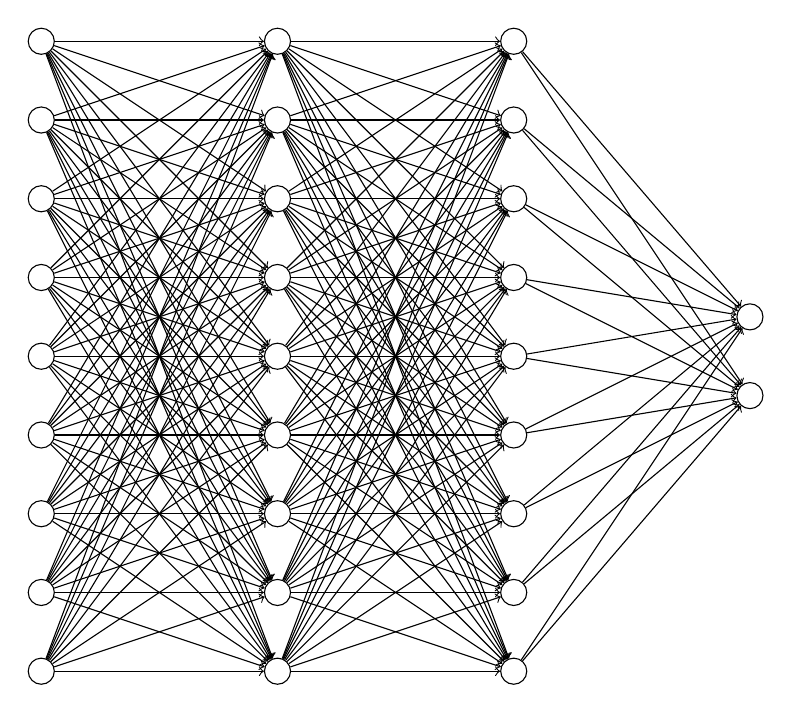
\begin{tikzpicture}[xscale = 3]
  \node[draw, circle] (N11) at (0, 0){
  };

  \node[draw, circle] (N21) at (0, -1){
  };

  \node[draw, circle] (N31) at (0, -2){
  };

  \node[draw, circle] (N41) at (0, -3){
  };

  \node[draw, circle] (N51) at (0, -4){
  };

  \node[draw, circle] (N61) at (0, -5){
  };

  \node[draw, circle] (N71) at (0, -6){
  };

  \node[draw, circle] (N81) at (0, -7){
  };

  \node[draw, circle] (N91) at (0, -8){
  };

  \node[draw, circle] (N12) at (1, 0){
  };

  \node[draw, circle] (N22) at (1, -1){
  };

  \node[draw, circle] (N32) at (1, -2){
  };

  \node[draw, circle] (N42) at (1, -3){
  };

  \node[draw, circle] (N52) at (1, -4){
  };

  \node[draw, circle] (N62) at (1, -5){
  };

  \node[draw, circle] (N72) at (1, -6){
  };

  \node[draw, circle] (N82) at (1, -7){
  };

  \node[draw, circle] (N92) at (1, -8){
  };

  \node[draw, circle] (N13) at (2, 0){
  };

  \node[draw, circle] (N23) at (2, -1){
  };

  \node[draw, circle] (N33) at (2, -2){
  };

  \node[draw, circle] (N43) at (2, -3){
  };

  \node[draw, circle] (N53) at (2, -4){
  };

  \node[draw, circle] (N63) at (2, -5){
  };

  \node[draw, circle] (N73) at (2, -6){
  };

  \node[draw, circle] (N83) at (2, -7){
  };

  \node[draw, circle] (N93) at (2, -8){
  };

  \node[draw, circle] (N14) at (3, -3.5){
  };

  \node[draw, circle] (N24) at (3, -4.5){
  };

  \draw[->] (N11) -- (N12);
  \draw[->] (N11) -- (N22);
  \draw[->] (N11) -- (N32);
  \draw[->] (N11) -- (N42);
  \draw[->] (N11) -- (N52);
  \draw[->] (N11) -- (N62);
  \draw[->] (N11) -- (N72);
  \draw[->] (N11) -- (N82);
  \draw[->] (N11) -- (N92);
  \draw[->] (N21) -- (N12);
  \draw[->] (N21) -- (N22);
  \draw[->] (N21) -- (N32);
  \draw[->] (N21) -- (N42);
  \draw[->] (N21) -- (N52);
  \draw[->] (N21) -- (N62);
  \draw[->] (N21) -- (N72);
  \draw[->] (N21) -- (N82);
  \draw[->] (N21) -- (N92);
  \draw[->] (N31) -- (N12);
  \draw[->] (N31) -- (N22);
  \draw[->] (N31) -- (N32);
  \draw[->] (N31) -- (N42);
  \draw[->] (N31) -- (N52);
  \draw[->] (N31) -- (N62);
  \draw[->] (N31) -- (N72);
  \draw[->] (N31) -- (N82);
  \draw[->] (N31) -- (N92);
  \draw[->] (N41) -- (N12);
  \draw[->] (N41) -- (N22);
  \draw[->] (N41) -- (N32);
  \draw[->] (N41) -- (N42);
  \draw[->] (N41) -- (N52);
  \draw[->] (N41) -- (N62);
  \draw[->] (N41) -- (N72);
  \draw[->] (N41) -- (N82);
  \draw[->] (N41) -- (N92);
  \draw[->] (N51) -- (N12);
  \draw[->] (N51) -- (N22);
  \draw[->] (N51) -- (N32);
  \draw[->] (N51) -- (N42);
  \draw[->] (N51) -- (N52);
  \draw[->] (N51) -- (N62);
  \draw[->] (N51) -- (N72);
  \draw[->] (N51) -- (N82);
  \draw[->] (N51) -- (N92);
  \draw[->] (N61) -- (N12);
  \draw[->] (N61) -- (N22);
  \draw[->] (N61) -- (N32);
  \draw[->] (N61) -- (N42);
  \draw[->] (N61) -- (N52);
  \draw[->] (N61) -- (N62);
  \draw[->] (N61) -- (N72);
  \draw[->] (N61) -- (N82);
  \draw[->] (N61) -- (N92);
  \draw[->] (N71) -- (N12);
  \draw[->] (N71) -- (N22);
  \draw[->] (N71) -- (N32);
  \draw[->] (N71) -- (N42);
  \draw[->] (N71) -- (N52);
  \draw[->] (N71) -- (N62);
  \draw[->] (N71) -- (N72);
  \draw[->] (N71) -- (N82);
  \draw[->] (N71) -- (N92);
  \draw[->] (N81) -- (N12);
  \draw[->] (N81) -- (N22);
  \draw[->] (N81) -- (N32);
  \draw[->] (N81) -- (N42);
  \draw[->] (N81) -- (N52);
  \draw[->] (N81) -- (N62);
  \draw[->] (N81) -- (N72);
  \draw[->] (N81) -- (N82);
  \draw[->] (N81) -- (N92);
  \draw[->] (N91) -- (N12);
  \draw[->] (N91) -- (N22);
  \draw[->] (N91) -- (N32);
  \draw[->] (N91) -- (N42);
  \draw[->] (N91) -- (N52);
  \draw[->] (N91) -- (N62);
  \draw[->] (N91) -- (N72);
  \draw[->] (N91) -- (N82);
  \draw[->] (N91) -- (N92);
  \draw[->] (N12) -- (N13);
  \draw[->] (N12) -- (N23);
  \draw[->] (N12) -- (N33);
  \draw[->] (N12) -- (N43);
  \draw[->] (N12) -- (N53);
  \draw[->] (N12) -- (N63);
  \draw[->] (N12) -- (N73);
  \draw[->] (N12) -- (N83);
  \draw[->] (N12) -- (N93);
  \draw[->] (N22) -- (N13);
  \draw[->] (N22) -- (N23);
  \draw[->] (N22) -- (N33);
  \draw[->] (N22) -- (N43);
  \draw[->] (N22) -- (N53);
  \draw[->] (N22) -- (N63);
  \draw[->] (N22) -- (N73);
  \draw[->] (N22) -- (N83);
  \draw[->] (N22) -- (N93);
  \draw[->] (N32) -- (N13);
  \draw[->] (N32) -- (N23);
  \draw[->] (N32) -- (N33);
  \draw[->] (N32) -- (N43);
  \draw[->] (N32) -- (N53);
  \draw[->] (N32) -- (N63);
  \draw[->] (N32) -- (N73);
  \draw[->] (N32) -- (N83);
  \draw[->] (N32) -- (N93);
  \draw[->] (N42) -- (N13);
  \draw[->] (N42) -- (N23);
  \draw[->] (N42) -- (N33);
  \draw[->] (N42) -- (N43);
  \draw[->] (N42) -- (N53);
  \draw[->] (N42) -- (N63);
  \draw[->] (N42) -- (N73);
  \draw[->] (N42) -- (N83);
  \draw[->] (N42) -- (N93);
  \draw[->] (N52) -- (N13);
  \draw[->] (N52) -- (N23);
  \draw[->] (N52) -- (N33);
  \draw[->] (N52) -- (N43);
  \draw[->] (N52) -- (N53);
  \draw[->] (N52) -- (N63);
  \draw[->] (N52) -- (N73);
  \draw[->] (N52) -- (N83);
  \draw[->] (N52) -- (N93);
  \draw[->] (N62) -- (N13);
  \draw[->] (N62) -- (N23);
  \draw[->] (N62) -- (N33);
  \draw[->] (N62) -- (N43);
  \draw[->] (N62) -- (N53);
  \draw[->] (N62) -- (N63);
  \draw[->] (N62) -- (N73);
  \draw[->] (N62) -- (N83);
  \draw[->] (N62) -- (N93);
  \draw[->] (N72) -- (N13);
  \draw[->] (N72) -- (N23);
  \draw[->] (N72) -- (N33);
  \draw[->] (N72) -- (N43);
  \draw[->] (N72) -- (N53);
  \draw[->] (N72) -- (N63);
  \draw[->] (N72) -- (N73);
  \draw[->] (N72) -- (N83);
  \draw[->] (N72) -- (N93);
  \draw[->] (N82) -- (N13);
  \draw[->] (N82) -- (N23);
  \draw[->] (N82) -- (N33);
  \draw[->] (N82) -- (N43);
  \draw[->] (N82) -- (N53);
  \draw[->] (N82) -- (N63);
  \draw[->] (N82) -- (N73);
  \draw[->] (N82) -- (N83);
  \draw[->] (N82) -- (N93);
  \draw[->] (N92) -- (N13);
  \draw[->] (N92) -- (N23);
  \draw[->] (N92) -- (N33);
  \draw[->] (N92) -- (N43);
  \draw[->] (N92) -- (N53);
  \draw[->] (N92) -- (N63);
  \draw[->] (N92) -- (N73);
  \draw[->] (N92) -- (N83);
  \draw[->] (N92) -- (N93);
  \draw[->] (N13) -- (N14);
  \draw[->] (N13) -- (N24);
  \draw[->] (N23) -- (N14);
  \draw[->] (N23) -- (N24);
  \draw[->] (N33) -- (N14);
  \draw[->] (N33) -- (N24);
  \draw[->] (N43) -- (N14);
  \draw[->] (N43) -- (N24);
  \draw[->] (N53) -- (N14);
  \draw[->] (N53) -- (N24);
  \draw[->] (N63) -- (N14);
  \draw[->] (N63) -- (N24);
  \draw[->] (N73) -- (N14);
  \draw[->] (N73) -- (N24);
  \draw[->] (N83) -- (N14);
  \draw[->] (N83) -- (N24);
  \draw[->] (N93) -- (N14);
  \draw[->] (N93) -- (N24);

\end{tikzpicture}

    }
  };

  \node (predTeacher) at (10, 2) {
    \scalebox{0.25}{
      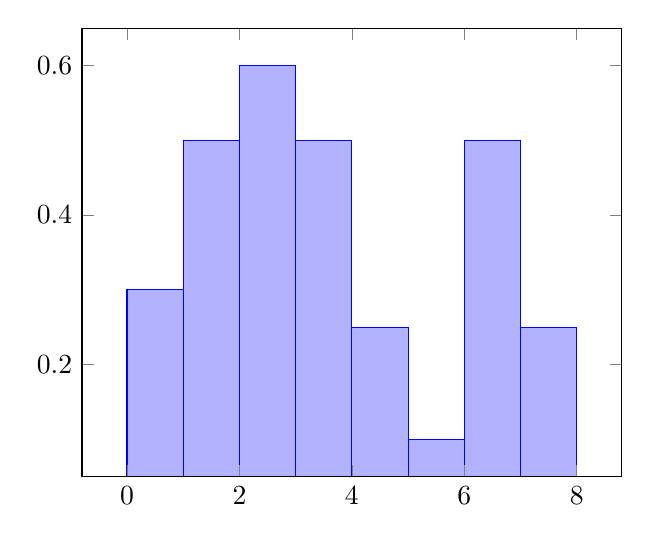
\begin{tikzpicture}
  \begin{axis}[
            area style,
            ]
    \addplot+[ybar interval,mark=no] plot coordinates {
      (0,.3)
      (1,.5)
      (2,.6)
      (3,.5)
      (4,.25)
      (5,.1)
      (6,.5)
      (7,.25)
      (8,.1)
    };
  \end{axis}
\end{tikzpicture}

    }
  };

  \node (predStudent) at (10, -2) {
    \scalebox{0.25}{
      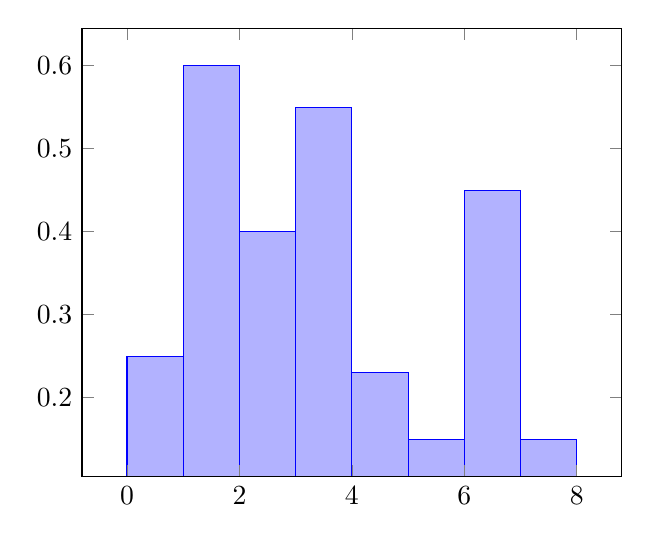
\begin{tikzpicture}
  \begin{axis}[
            area style,
            ]
    \addplot+[ybar interval,mark=no] plot coordinates {
      (0,.25)
      (1,.6)
      (2,.4)
      (3,.55)
      (4,.23)
      (5,.15)
      (6,.45)
      (7,.15)
      (8,.18)
    };
  \end{axis}
\end{tikzpicture}

    }
  };

  \draw[->, thick] (cleanImage) -- node [below = 0.05cm] {\rotatebox{-35}{\tiny pertubation}} (perturbedImage);
  \draw[->, thick] (cleanImage) -- (teacher);
  \draw[->, thick] (perturbedImage) -- (student);
  \draw[->, thick] (teacher) -- (predTeacher);
  \draw[->, thick] (student) -- (predStudent);
  \draw[<->, thick] (predTeacher) -- node [left = 0.3cm] {\small Consistency loss (MSE, KL div)} (predStudent);
\end{tikzpicture}

  \end{center}

  \bigskip

  We do not need a label for the clean image, we want to teach the
  model to be \textcolor{blue}{noise invariant}.

\end{frame}
%%%%%%%%%%%%%%%%%%%%%%%%%%%%%%%%%%%%%%%%%%%%%%%%%%%%%%%%%%%%%%%%%%%%%%

%%%%%%%%%%%%%%%%%%%%%%%%%%%%%%%%%%%%%%%%%%%%%%%%%%%%%%%%%%%%%%%%%%%%%%
\begin{frame}
  \frametitle{Conclusion}

  \begin{enumerate}
    \item Establish a baseline using basic algorithms (naive Bayes,
      logistic regression, random forest, etc.).
      \medskip
    \item Choose a model architecture (MLP, CNN, RNN, Transformer).
      \medskip
    \item Try to find (or build) a pre-trained version of this model
      that performs a related task and retrain it to your
      problem (\emph{transfer learning}).
      \medskip
    \item Try to find a related auxiliary task to regularize to
      improve the model learning abilities. (\emph{multi-task
        learning}).
      \medskip
    \item Once the performance of the model is relatively good, try to
      use unlabelled data to improve performances
      (\emph{semi-supervised learning}).
  \end{enumerate}
\end{frame}
%%%%%%%%%%%%%%%%%%%%%%%%%%%%%%%%%%%%%%%%%%%%%%%%%%%%%%%%%%%%%%%%%%%%%%

%%%%%%%%%%%%%%%%%%%%%%%%%%%%%%%%%%%%%%%%%%%%%%%%%%%%%%%%%%%%%%%%%%%%%%
\begin{frame}
  \frametitle{References}

  \fontsize{6pt}{7.2}\selectfont

  \begin{itemize}
  \item \href{https://blog.slavv.com/a-gentle-intro-to-transfer-learning-2c0b674375a0}{https://blog.slavv.com/a-gentle-intro-to-transfer-learning-2c0b674375a0}
  \item Radford, Alec, et al. "Improving language understanding by generative pre-training." URL
    \href{https://s3-us-west-2.amazonaws.com/openai-assets/research-covers/language-unsupervised/language_understanding_paper.pdf}{Article pdf link}
    \href{https://blog.openai.com/language-unsupervised/}{Blog post} (2018).
  \item Devlin, Jacob, et al. "Bert: Pre-training of deep
    bidirectional transformers for language understanding." arXiv
    preprint arXiv:1810.04805 (2018).
  \item Poplin, Ryan, et al. "Predicting cardiovascular risk factors
    from retinal fundus photographs using deep learning."  arXiv
    preprint arXiv:1708.09843 (2017).
  \item Kaiser, Lukasz, et al. "One model to learn them all."  arXiv
    preprint arXiv:1706.05137 (2017).
  \item Tarvainen, Antti, et al. "Mean teachers are better
    role models: Weight-averaged consistency targets improve
    semi-supervised deep learning results." Advances in neural
    information processing systems (2017).
  \item Miyato, Takeru, et al. "Virtual adversarial training: a
    regularization method for supervised and semi-supervised
    learning." IEEE transactions on pattern analysis and machine
    intelligence (2018).
  \end{itemize}
\end{frame}
%%%%%%%%%%%%%%%%%%%%%%%%%%%%%%%%%%%%%%%%%%%%%%%%%%%%%%%%%%%%%%%%%%%%%%

\end{document}
